\chapter{A Precise Half-Wave Rectifier: Part II}


\section{Objectives}
\begin{itemize}
    \item To verify one precise full-wave rectifier
\end{itemize}

\section{Materials}
\begin{itemize}
    \item Breadboard
    \item DC power supply
    \item Digital Multi-Meter
    \item \hyperref[1N4148]{Diode (1N4148)}
    \item Function Generator
    \item \hyperref[LM741_1]{Op.Amp. (LM741)}
    \item Oscilloscope
    \item Resistors
\end{itemize}

\section{Introduction}
    \subsection{Circuit Diagram}
    \begin{figure}[h]
        \centering
        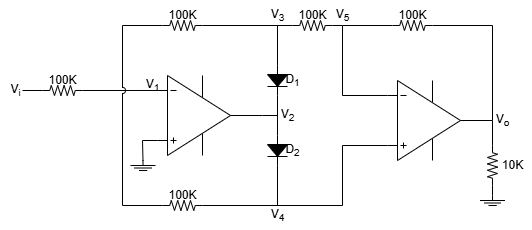
\includegraphics[width=0.7\linewidth]{Lab14/Lab14.drawio.png}
        \caption{Circuit Diagram}
        \label{l14f}
    \end{figure}
    \FloatBarrier

\section{Detailed Procedures}
    \subsection{Analyzation}
    First, we analyze the relationship between $V_i$ and $V_o$ in the circuits.\par
    \begin{itemize}
        \item $V_i > 0, D_1~\text{on}, D_2~\text{off}$\par
            \begin{equation}
                \begin{cases}
                    V_1=0\\
                    V_5=V_4=0\\
                    \frac{V_i-0}{100k} = \frac{0-V_3}{100k}\\
                    \frac{V_3-0}{100k} = \frac{0-V_0}{100k}\\
                \end{cases}
                \label{l14eq1}
            \end{equation}
            From Equation.\ref{l14eq1} and given data, we can obtain\par
            \begin{equation*}
                \begin{cases}
                    V_o=-V_3=V_i\\
                    V_1=0\\
                    V_2=-V_i-V_\gamma\\
                    V_3=-V_i\\
                    V_5=V_4=0\\
                    -V_i-V_\gamma > -10\\
                \end{cases}
            \end{equation*}
            For the first Op.Amp., $0<V_i<10-V_\gamma(9.3)$.\\
            For the second Op.Amp., $V_i<10$\\
        \item $V_i < 0, D_1~\text{off}, D_2~\text{on}$
            \begin{equation}
                \begin{cases}
                    V_1=0\\
                    V_4=V_5=-\frac{2}{3}V_i\\
                    \frac{V_i-0}{100k}=\frac{0-V_4}{100k}+\frac{0-V_5}{100k}\\
                    V_2=V_4+V_\gamma=-\frac{2}{3}V_i+V_\gamma\\
                    V_3=-\frac{V_5}{2}=-\frac{1}{3}V_i\\
                    \frac{0-V_5}{200k}=\frac{V_5-V_o}{100k}\\
                \end{cases}
                \label{l14eq2}
            \end{equation}
            From Equation.\ref{l14eq2} and given data, we can obtain\par
            \begin{equation*}
                \begin{cases}
                V_o=\frac{3}{2}V_5=-V_i\\
                V_1=0\\
                V_2=-\frac{2}{3}V_i+V_\gamma\\
                V_3=-\frac{1}{3}V_i\\
                V_4=V_5=-\frac{2}{3}V_i\\
                -V_i<10\\
                \end{cases}
            \end{equation*}
            For the first Op.Amp., $V_i>\frac{3}{2}(-10+V_\gamma)$.\\
            For the second Op.Amp., $V_i>-10$\\
    \end{itemize}
    \FloatBarrier
    
    \subsection{Procedures}
    
    
\section{Discussion}


\section{Conclusion}